\subsection*{Actividad 1.2}

El problema propone un cilindro con la siguiente descripción:

\begin{center}
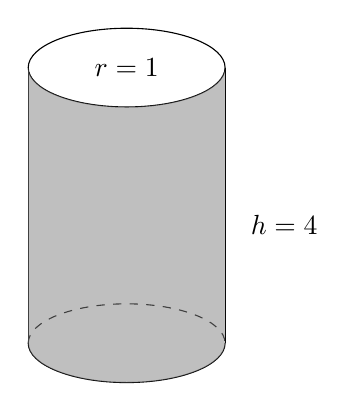
\begin{tikzpicture}
\draw (0,0) ellipse (1.25 and 0.5);
\draw (-1.25,0) -- (-1.25,-3.5);
\draw (-1.25,-3.5) arc (180:360:1.25 and 0.5);
\draw [dashed] (-1.25,-3.5) arc (180:360:1.25 and -0.5);
\draw (1.25,-3.5) -- (1.25,0);  
\fill [gray,opacity=0.5] (-1.25,0) -- (-1.25,-3.5) arc (180:360:1.25 and 0.5) -- (1.25,0) arc (0:180:1.25 and -0.5);
\draw (2,-2) node{$h = 4$};
\draw (0,0) node{$r = 1$};
\end{tikzpicture}
\end{center}

El volumen del agua en función de la altura sigue el modelo $V(h) = 4\pi h$. 

La tasa media del volumen entre los puntos $[2,2.5]$ es:

\begin{align*}
    V_m &= \frac{V_{(2,5)} - V_{(2)}}{2,5-2}\\
    V_m &= \frac{4\pi\frac{5}{2} - 4\pi 2}{\frac{5}{2}-2}\\
    V_m &= 4\pi
\end{align*}

Dados dos puntos cualesquiera, $a$ y $b$, llegamos a la siguiente expresión:

\begin{align*}
    V_m &= \frac{V_{(b)} - V_{(a)}}{b-a}\\
    V_m &= \frac{4\pi b - 4\pi a}{b-a}\\
    V_m &= \frac{4\pi \cancel{(b - a)}}{\cancel{b-a}}\\
    V_m &= 4\pi
\end{align*}

Con ello podemos concluir que, a diferencia de lo que ocurría en el modelo anterior, en este caso la pendiente permanece constante a lo largo de la función, por lo cual la velocidad media es un mejor indicador del cambio en la función.